%% bulk_genome_comparisons_expt.tex
%% Author: Leighton Pritchard
%% Copyright: James Hutton Institute
%% Bulk genome comparisons - experimental

%
\begin{frame}
  \frametitle{Bulk genome comparisons}
  \Large{
    \textcolor{olive}{
      \textbf{
      You don't have to sequence genomes to compare them \\
      (but it helps)
      }
    }
  }
\end{frame}

%
\begin{frame}
  \frametitle{Genome comparisons predate NGS}
  \begin{itemize}
    \item Sequence data wasn't always cheap and abundant
    \item Practical, experimental genome comparisons were needed
  \end{itemize}
  \begin{center}
    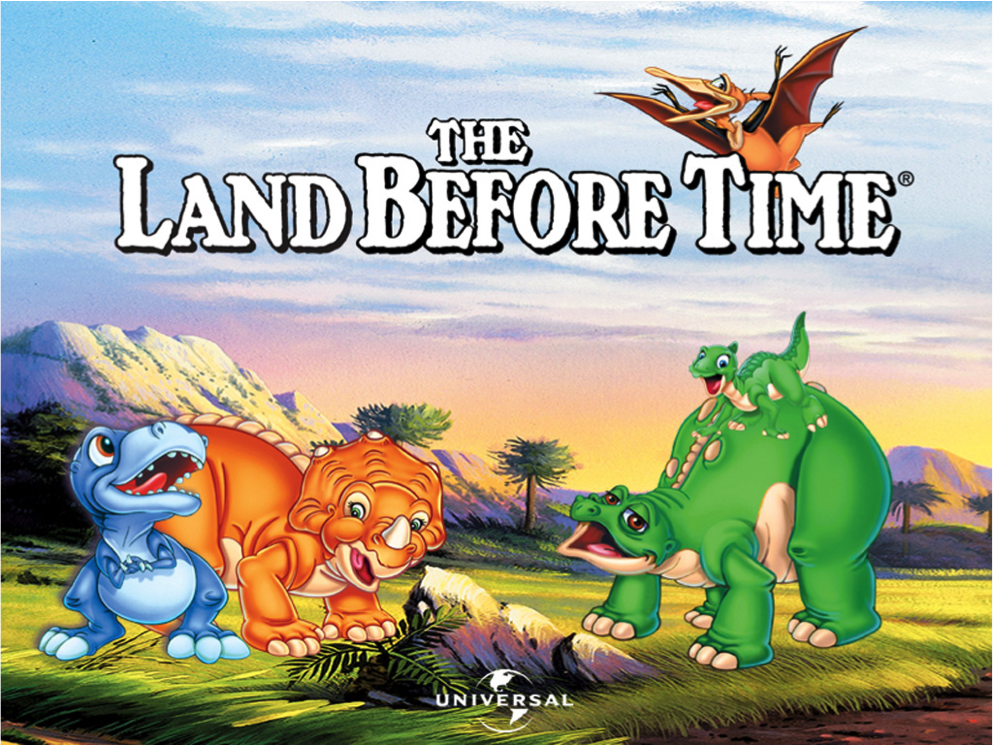
\includegraphics[width=0.7\textwidth]{images/land_before_time}
  \end{center}  
\end{frame}

%
\begin{frame}
  \frametitle{Bulk genome comparisons}
  \Large{
    \textcolor{olive}{
      \textbf{
      Calculate values for individual genomes, \\
      then compare them.
      }
    }
  }
\end{frame}

%
\begin{frame}
  \frametitle{Bulk genome properties}
    \begin{itemize}
      \item Large-scale summary measurements
      \item Measure genomes independently - compare values later
        \begin{itemize}
         \item<2-2> \textcolor{red}{What kinds of measurements/properties?}
         \item<3-> \textcolor{hutton_green}{Number of chromosomes}
         \item<3-> \textcolor{hutton_blue}{Ploidy}
         \item<3-> \textcolor{RawSienna}{Chromosome size}
         \item<3-> \textcolor{hutton_purple}{Nucleotide (A,C,G,T) frequency}        
        \end{itemize}
    \end{itemize}
\end{frame}

%
\begin{frame}
  \frametitle{Chromosome count/size
%    \footnote{\tiny{Kamisugi \textit{et al}. (1993) \textit{Chromosome Res.} \textbf{1}(3): 189-196
%}}
%    \footnote{\tiny{\href{http://dx.doi.org/10.1038/nrg3375
%}{Wang \textit{et al}. (2013) \textit{Nat. Rev. Genet.} doi:10.1038/nrg3375
%}}}
  }
    \begin{itemize}
      \item chromosome count and ploidy can vary widely \\
        \begin{table}
		  \begin{tabular}{l | c | c }
		    Organism & Chromosomes & Ploidy  \\
			\hline \hline
			\textit{E. coli} & 1 & 1  \\ 
			Human (\textit{H. sapiens}) & 46 & 2 \\
			\hline
			Rice (\textit{O. sativa}) & 24 & 1  \\
			Adders-tongue & & \\ 
			(\textit{Ophioglossum reticulatum}) & 1260 & 84 \\
			\hline
			Domestic (not wild) wheat somatic & 42 & 6 \\
			Domestic (not wild) wheat gametic & 14 & 2 \\			
		  \end{tabular}
		\end{table}
	\end{itemize}
  \begin{center}
    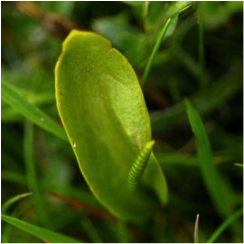
\includegraphics[height=0.2\textheight]{images/adders_tongue}
  \end{center}  		
\end{frame}